\documentclass[12pt, letterpaper]{article}
\usepackage[utf8]{inputenc}
 \usepackage[letterpaper, margin=0.8in]{geometry}
 \usepackage{amssymb}
\usepackage{amsmath}
 \usepackage{enumitem}
\usepackage {listings}
\usepackage{pgfplots}
\usepgfplotslibrary{external}
\usepackage{graphicx}

\title{CS425 Project 4(Report)\\Back-Propogation}
\author{Ksenia Burova}
\date{November \(20^{th}\), 2017}

\begin{document}
\maketitle

\noindent {\bf Abstract:} In this project, the goal was to implement and examine multilayer artificial neural networks (ANNs) and explore back-propagation learning algorithm by applying it to spam classification problem. The task was simply to classify given data instances as spam or not. After implementing training and testing functions, we had to make observations on how different parameters for building networks, like number of hidden layers, number of nodes (neurons), number of epochs and learning rate would affect training, validation and testing performance. For performance analysis results were displayed in several plots.

\begin{enumerate}[label=\Roman*.]
	{\bf \item Introduction.} \\
	
	Feed forward artificial networks have such property that no sequence of connections among neurons forms a cycle, so basically, no neuron can feed back to itself. Thus information, flows only one direction, from input neurons all the way to the output nodes. Perceptron, pattern classification device, is a great example of feed-forward neural net. \\
	{\center 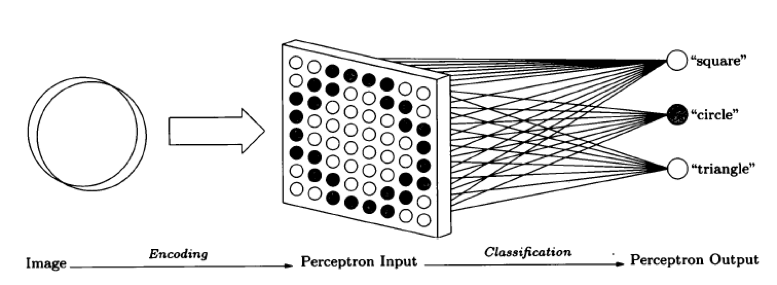
\includegraphics[scale=1]{1.png} \\}
	Perceptron demonstrates how image encoding and classification goes one direction. here are single-layer and multiple-layer perceptron kinds of neural network. Single-layer one have inputs and outputs only, whereas multiple-layer also have one or more hidden layers in between.\\
	
	{\bf \item Back-Propogation.} \\
	
	Back-propagation algorithm is the most commonly used for training multi-layer neural networks. The general idea behind this algorithm is run several data sets, compare output with expected value and compute the predefined error function. Then error function is fed back through the network and used for adjustment of all the weights to minimize the value of the error function. Such operation is done several number of times until error is minimized to almost zero value, which indicates that network is trained and should solve testing problems correctly. Let's look at the example with using logistic sigmoid for output layer.\\
	
	So, as it's been said, first we propagate input values forward through the network:
	{\center 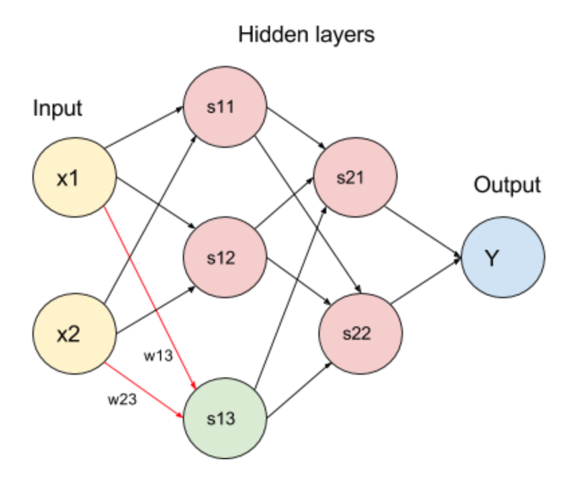
\includegraphics[scale=.9]{2.png} \\}
	
	Next, we start with two inputs and propagate through two hidden layers before calculating the output. We calculate sigmoidal function \(g(x) = \frac{1}{1 + exp(-x)}\) value for each node, where \(x\) is determined by summation of products of all weights (coming into a node) and \(s_{ij}\) values from previous layer corresponding to those weights. We also add bias weight to it for weigh correction. So, we get \( x_k = \sum\limits_{i=0}^{prevNodesNum} s_{ij}w_{ik}+b_k \). So, in our example, we do \(x = x_1w_{13} + x_2w_{23} + biasWeight\). And then calculate \(g(x)\) for node colored in green, which is sigma value that is used in calculations for nodes in next layer. \\
	
	{\center 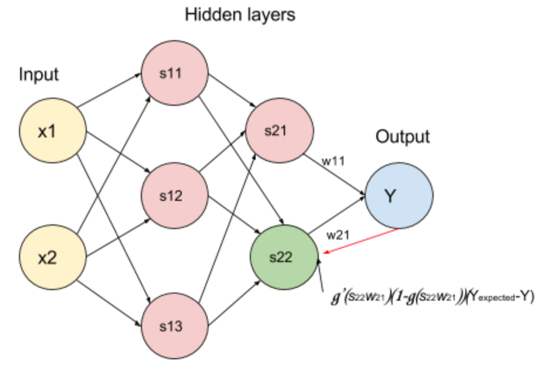
\includegraphics[scale=1]{3.png} \\}
	{\center 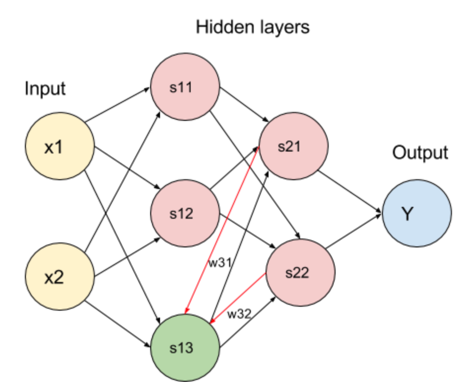
\includegraphics[scale=1]{4.png} \\}
	
	After output is computed, we calculate the error function \(\delta\) value. First layer in the end will take in account the difference between expected output and received one. And for every other node, we calculate \( \delta_{s_{ij}} = g'(x_{ij})\sum_kw_{kj}\delta_{s_{i+1,j}} \). As we can see, delta function is from layer before is used for calculation of delta function for current node. Calculating the derivative of the sigmoidal function gives us information about how the output changes when the input changes. If its value is too large that means the input was near its threshold and little change may change  \(g(x)\), if it's too small, then value of \(g(x)\) is really close to 0 or 1. Also, the sign of \(g'(x)(t-y)\) will tell us which way neuron was wrong. Overall, this term will give us all the information needed for error correction. We use delta function and learning rate value for computing adjusted weight.
	{\bf \item Project Data.} \\
	
	 In this project, we were given a file {\it spambase.data} which had 58 attributes:
	 \begin{itemize}
	 	\item 48 continuous real [0,100] attributes of type word\_freq\_WORD (percentage of words in the e-mail that match WORD)
		\item 6 continuous real [0,100] attributes of type char\_freq\_CHAR (percentage of characters in the e-mail that match CHAR)
		\item 1 continuous real [1,...] attribute of type capital\_run\_length\_average (average length of uninterrupted sequences of capital letters)
		\item 1 continuous integer [1,...] attribute of type capital\_run\_length\_longest (length of longest uninterrupted sequence of capital letters)
		\item 1 continuous integer [1,...] attribute of type capital\_run\_length\_total (total number of capital letters in the e-mail)
		\item Class: (0 - no spam, 1 -  spam)
	\end{itemize}
	
	There were no missing values in data but data values range is different for some attributes. Because of that I decided to normalize data. Without standardization my program would fail to run or would give me really bad results.
	I've placed all continuous values of the data into multidimensional array called {\bf dataFeatures}, and kept classes in one-dimensional array called {\bf dataLabels} for simplicity of implementation. During experiments, data was split into 3 sets: training, validation and testing. I used 60/20/20 proportion rule for splitting the data. 
		
	{\bf \item Tools and Program.}\\
	
	I've used {\bf python} programming language, {\bf numpy} library for arithmetic, {\bf sklearn} library for splitting my data into training, validation and testing datasets, and {\bf matplotlib} library to built plots for this project. I have a program named {\bf abckprop.py} , that includes 2 classes: {\bf Data} for normalizing and constructing data sets, and {\bf BackProp} that has back propagationimplementation. I've split the algorithm into several functions:
	\begin{itemize}
		\item compute\_outputs(): forward propagation
		\item compute\_delta(): consruct delta for back propagation
		\item update\_weights(): propagate backwards
		\item train\_network()
		\item validate\_network()
		\item test\_network()
		\item plot\_RMSE()
		\item run(): for given number of epochs it trains and validates network, saves rmse values for each epoch, plots results and tests network
	\end{itemize}
	
	In my main function, I've listed following layer-neurons , epochs and learning rate combinations:
	\begin{verbatim}
	    layers = [ [10],
               [30],
               [65],
               [58],
               [100],
               [10, 10],
               [60, 40],
               [30, 30],
               [58, 58],
               [58, 58, 58],
               [60, 70, 80],
               [30, 40, 30],
               [60, 100, 60],
               [15, 15, 15],
               [10, 10, 10, 10],
               [60, 70, 70, 60],
               [60, 100, 40, 30],
               [60, 40, 30, 50],
               [10, 10, 10, 10, 10],
               [60, 60, 60, 60, 60],
               [60, 70, 100, 70, 60]]
               
    epochs = [6, 10, 30, 60, 200, 800, 2000, 5000]
    lrate = [0.01, 0.1, 0.25, 0.4, 0.65, 0.8, 0.9, 1.0]
	\end{verbatim}
	 I mix and match all these to find out which combination is the best.
	 
	{\bf \item Performance metrics.}\\
	
	To evaluate performance of  classification algorithms, we have to compare correct classifications with our classifications on evaluation data sets after algorithm is run. We are going to calculate and look at the following values: 
	\begin{itemize}
		\item Confusion Matrix \\
		{\center 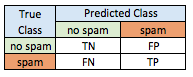
\includegraphics[scale=1]{5.png} \\}
		where TP = \# true positives, TN = \# true negatives, FP = \# false positives, FN = \# false negatives.\\
		\item Accuracy = (TN + TP) / (TN + TP + FN + FP)\\
		{\bf Accuracy} tells us what percent of data was classified correctly. \\
		\item TPR (true positive rate, recall, or sensitivity) = TP / (TP + FN)\\
		{\bf Sensitivity} shows us rate at which true positives are not missed/overlooked \\
		\item PPV (positive predictive value or precision) = TP / (TP + FP)\\
		{\bf Precision} is basically a fraction of relevant positive data from all the positive data we have, meaning have many of those classified as spam are really spam e-emails. \\ 
		\item TNR (true negative rate or specificity) = TN / (TN + FP)\\
		{\bf Specificity} is a rate that shows how well we can distinguish data that is truly negative, meaning that e-mail is not spam.\\
		\item F Score = PPV * TPR / (PPV + TPR)\\
		{\bf F score} is a harmonic average of precision and sensitivity, it is basically used if we can't decide with of 2 metrics to use for performance measurements. \\
	\end{itemize}
	
	{\bf \item Experiment Observations. }\\
	
	
	{\bf \item Conclusions.}\\
	
\end{enumerate}
\end{document}
	
	
	
	
	
	
